\documentclass[aspectratio=169]{beamer}

\usetheme{durham}

\usepackage{booktabs}
\usepackage{array}
\usepackage{hyperref}
\usepackage{graphicx}
\usepackage{tikz}
\usepackage{pgfplots}
\pgfplotsset{compat=1.18}
\usetikzlibrary{arrows.meta,backgrounds,calc,fit,positioning}

\title[Filipino OmniVoice Fine-Tuning]{Filipino Adaptation of OmniVoice for Voice Cloning and Text-to-Speech}
\subtitle{Final Project Presentation}
\author{}
\institute{}
\date{\today}
\setbeamertemplate{footline}{}

\begin{document}

\maketitle

\begin{frame}{The Problem}
  Voice cloning systems synthesize speech in a target speaker's voice from a short reference audio.

  \vspace{0.6em}

  \begin{itemize}
    \item High-quality voice cloning is strongest in high-resource languages.
    \item Filipino speech AI remains low-resource, with few open Filipino workflows.
    \item OmniVoice supports Filipino, but with only about \textbf{7.71 hours} of Filipino in its training mixture.
    \item The UP-DSP Philippine Languages Database holds almost \textbf{49 hours} of Filipino speech.
  \end{itemize}

  \vspace{0.6em}
  \begin{block}{What We Did}
    Fine-tune OmniVoice on curated Filipino speech and measure whether the adapted model is better than the base model.
  \end{block}
\end{frame}

\begin{frame}{Background: OmniVoice}
  \begin{columns}[T]
    \begin{column}{0.38\textwidth}
      
\includegraphics[height=0.66\textheight,keepaspectratio]{\detokenize{../../images/omnivoice paper.png}}
    \end{column}
    \begin{column}{0.58\textwidth}
      \begin{itemize}
        \item Open-source multilingual zero-shot TTS and voice cloning model.
        \item Supports 600+ languages, including Filipino (\texttt{fil}).
        \item Generates discrete acoustic tokens with a masked-token (diffusion language model) process.
        \item Provides official fine-tuning and evaluation scripts.
        \item Practical to adapt instead of training a Filipino model from scratch.
      \end{itemize}
      \vspace{0.5em}
      \small Source: Zhu et al. (2026).
    \end{column}
  \end{columns}
\end{frame}

\begin{frame}{Research Question}
  \begin{block}{Main Research Question}
    How much does Filipino-specific fine-tuning improve OmniVoice for Filipino TTS and voice cloning across intelligibility, naturalness, and speaker similarity metrics?
  \end{block}

  \vspace{0.5em}

  \begin{itemize}
    \item Model: \texttt{k2-fsa/OmniVoice}, adapted with supervised fine-tuning.
    \item Data: Filipino read speech from the UP-DSP Philippine Languages Database.
    \item Compute: free Kaggle T4 GPU notebooks.
    \item Baseline: the unmodified pretrained OmniVoice checkpoint.
    \item Tracking: all runs logged in Weights and Biases.
  \end{itemize}
\end{frame}

\begin{frame}{Dataset: UP-DSP Philippine Languages Database}
  \begin{columns}[T]
    \begin{column}{0.48\textwidth}
      
\includegraphics[width=\linewidth,height=0.62\textheight,keepaspectratio]{\detokenize{../../images/up dsp philippine languages database.png}}
    \end{column}
    \begin{column}{0.48\textwidth}
      \begin{itemize}
        \item Released through Mozilla Data Collective (CC-BY-NC-4.0).
        \item WAV audio with LOG transcript files.
        \item Filipino subset: 135 speakers, 52,879 utterances, 48:56:36.
        \item We used read speech only: the transcript reliably matches the audio.
      \end{itemize}
      \vspace{0.4em}
      \small Source: Cajote et al. (2024).
    \end{column}
  \end{columns}
\end{frame}

\begin{frame}{Data Preparation}
  Conservative filtering: read speech only, no transcripts with digits or parentheses, no broken WAVs, clips between 1 and 15 seconds, speaker-disjoint splits.

  \vspace{0.6em}

  \begin{table}
    \centering
    \small
    \begin{tabular}{lrrrr}
      \toprule
      Split & Samples & Percent & Hours & Speakers \\
      \midrule
      Train & 33,448 & 79.1\% & 31.9 & 103 \\
      Development & 4,506 & 10.7\% & 3.7 & 13 \\
      Test & 4,322 & 10.2\% & 4.2 & 13 \\
      \midrule
      Total & 42,276 & 100\% & 39.8 & 129 \\
      \bottomrule
    \end{tabular}
  \end{table}

  \vspace{0.5em}
  \small The 31.9 training hours are about \textbf{4$\times$} the Filipino hours in OmniVoice's original training mixture. Domains include news, medical sentences, stories, greetings, proverbs, and many isolated-word prompts.
\end{frame}

\begin{frame}{System Architecture}
  \centering
  \scriptsize
  \resizebox{0.98\linewidth}{!}{\definecolor{archink}{HTML}{172033}
\definecolor{archmuted}{HTML}{64748B}
\definecolor{archdatafill}{HTML}{E8F7F0}
\definecolor{archdataedge}{HTML}{1F9D68}
\definecolor{archtrainfill}{HTML}{EEF2FF}
\definecolor{archtrainedge}{HTML}{5B6EE1}
\definecolor{archtokenfill}{HTML}{F8FAFC}
\definecolor{archmaskfill}{HTML}{334155}
\definecolor{archevalfill}{HTML}{E7F8FA}
\definecolor{archevaledge}{HTML}{1698A7}
\definecolor{archdeployfill}{HTML}{FFF1DF}
\definecolor{archdeployedge}{HTML}{F38020}
\colorlet{archslate}{archmuted!75}

\begin{tikzpicture}[
  font=\sffamily,
  nodeBox/.style={rectangle, rounded corners=7pt, align=center, minimum height=1.1cm, text width=3.2cm, line width=0.75pt, text=archink},
  smallBox/.style={rectangle, rounded corners=5pt, align=center, minimum height=0.85cm, text width=2.6cm, line width=0.65pt, font=\sffamily\scriptsize, text=archink},
  dataBox/.style={nodeBox, fill=archdatafill, draw=archdataedge},
  trainBox/.style={nodeBox, fill=archtrainfill, draw=archtrainedge},
  evalBox/.style={smallBox, fill=archevalfill, draw=archevaledge},
  deployBox/.style={smallBox, fill=archdeployfill, draw=archdeployedge},
  note/.style={font=\sffamily\scriptsize, text=archmuted, align=center},
  phaseTitle/.style={font=\sffamily\bfseries\small},
  arrow/.style={-{Latex[length=2.3mm]}, line width=0.95pt, draw=archink},
  dashArrow/.style={-{Latex[length=2.2mm]}, dashed, line width=0.85pt, draw=archmuted},
  biArrow/.style={{Latex[length=2.3mm]}-{Latex[length=2.3mm]}, line width=0.95pt, draw=archink}
]

\begin{scope}[on background layer]
  \filldraw[draw=archdataedge!70, fill=archdatafill!40, dashed, rounded corners=8pt, line width=0.7pt]
    (0.7, -0.4) rectangle (15.5, -3.0);
  \node[phaseTitle, text=archdataedge, anchor=north west] at (0.8, -0.6) {1. Dataset preparation};

  \filldraw[draw=archtrainedge!70, fill=archtrainfill!40, dashed, rounded corners=8pt, line width=0.7pt]
    (0.7, -3.1) rectangle (19.3, -7.55);
  \node[phaseTitle, text=archtrainedge, anchor=north west] at (0.8, -3.3) {2. Tokenization and supervised fine-tuning};

  \filldraw[draw=archevaledge!70, fill=archevalfill!40, dashed, rounded corners=8pt, line width=0.7pt]
    (0.7, -7.7) rectangle (19.3, -11.75);
  \node[phaseTitle, text=archevaledge, anchor=north west] at (0.8, -7.9) {3. Held-out evaluation and delivery};
\end{scope}

\node[dataBox] (raw)   at (2.8, -2.0) {\textbf{PLD Filipino}\\WAV audio +\\LOG transcripts};
\node[dataBox] (clean) at (8.15, -2.0) {\textbf{Cleaning}\\read speech only\\1.0s--15.0s};
\node[dataBox] (split) at (13.5, -2.0) {\textbf{Speaker-disjoint}\\train / dev / test\\JSONL splits};

\draw[arrow] (raw) -- (clean);
\draw[arrow] (clean) -- (split);

\node[trainBox] (tokenizer) at (2.8, -5.9) {\textbf{Higgs Audio v2}\\continuous waveform\\to discrete tokens};

\coordinate (gridOrigin) at (6.25, -6.46);
\coordinate (textOrigin) at ($(gridOrigin)+(0.4, 1.35)$);

\node[font=\sffamily\scriptsize\bfseries, text=archink] (gridTitle) at (8.15, -4.3) {8-codebook acoustic tokens};

\node[note, anchor=south east] at ($(gridOrigin)+(-0.08, 0.6)$) {8\\layers};
\node[note, anchor=north west] at ($(gridOrigin)+(3.88, 0.52)$) {masked\\target};
\node[note, anchor=west] at ($(textOrigin)+(3.4, 0.14)$) {text};

\foreach \x in {0,...,7} {
  \draw[fill=archdeployfill, draw=archdeployedge!80, rounded corners=0.5pt] ($(textOrigin)+(\x*0.38,0)$) rectangle ++(0.31,0.28);
}

\foreach \y in {0,...,7} {
  \foreach \x in {0,...,11} {
    \pgfmathtruncatemacro{\m}{mod(2*\x+\y,5)}
    \ifnum\m=0
      \draw[fill=archmaskfill, draw=archmaskfill, rounded corners=0.5pt] ($(gridOrigin)+(\x*0.32,\y*0.14)$) rectangle ++(0.25,0.095);
    \else
      \draw[fill=archtokenfill, draw=archslate, rounded corners=0.5pt] ($(gridOrigin)+(\x*0.32,\y*0.14)$) rectangle ++(0.25,0.095);
    \fi
  }
}

\node[trainBox] (omni) at (13.5, -5.9) {\textbf{OmniVoice}\\pretrained\\multilingual TTS\\masked diffusion LM};

\node[smallBox, fill=archtrainfill, draw=archtrainedge, inner sep=4pt, text width=2.8cm] (sft)  at (17.5, -5.1) {\textbf{SFT objective}\\weighted cross-entropy};
\node[smallBox, fill=archtrainfill, draw=archtrainedge, inner sep=4pt, text width=2.8cm] (ckpt) at (17.5, -6.7) {\textbf{Best-dev}\\checkpoint selection\\LR comparison};

\draw[arrow] (split.south) -- (omni.north);
\draw[arrow] (tokenizer.east) -- ($(gridOrigin)+(0, 0.56)$);
\draw[arrow] ($(gridOrigin)+(3.84, 0.56)$) -- (omni.west);
\draw[arrow] (omni.east) -- (sft.west);
\draw[arrow] (omni.east) -- (ckpt.west);

\node[evalBox] (infer) at (2.8, -9.9) {\textbf{Zero-shot inference}\\matched test prompts\\+ reference voices};
\node[evalBox] (gen)   at (6.4, -9.9) {\textbf{Generated}\\Filipino speech};

\node[evalBox] (wer) at (10.0, -8.9) {\textbf{Whisper ASR}\\WER};
\node[evalBox] (sim) at (10.0, -9.9) {\textbf{ECAPA-TDNN}\\SIM-o};
\node[evalBox] (mos) at (10.0, -10.9) {\textbf{UTMOS}\\naturalness};

\node[deployBox] (react) at (13.5, -9.9) {\textbf{React audio}\\showcase};

\node[deployBox] (cf) at (17.5, -9.9) {
  \begin{tabular}{@{}c@{\hspace{4pt}}c@{}}
    \begin{tikzpicture}[baseline=-0.6ex, scale=0.8]
      \fill[archdeployedge] (-0.15,-0.05) circle (0.08);
      \fill[archdeployedge] (0,0) circle (0.12);
      \fill[archdeployedge] (0.15,-0.05) circle (0.08);
      \fill[archdeployedge] (-0.15,-0.1) rectangle (0.15,-0.02);
    \end{tikzpicture} &
    \begin{tabular}{@{}c@{}}\textbf{Cloudflare}\\Workers\end{tabular}
  \end{tabular}
};

\draw[biArrow] (infer.east) -- (gen.west);

\draw[arrow] (gen.east) -- (wer.west);
\draw[arrow] (gen.east) -- (sim.west);
\draw[arrow] (gen.east) -- (mos.west);

\draw[arrow] (wer.east) -| (react.north);
\draw[arrow] (sim.east) -- (react.west);
\draw[arrow] (mos.east) -| (react.south);

\draw[arrow] (react.east) -- (cf.west);

\draw[dashArrow] (ckpt.south) -- (17.5, -9.75);
\node[note, anchor=west] at (17.8, -8.2) {selected checkpoint};

\end{tikzpicture}
}
\end{frame}

\begin{frame}{Fine-Tuning Setup}
  \begin{itemize}
    \item Environment: Kaggle notebooks, 2$\times$ NVIDIA T4, FP16, SDPA attention, gradient accumulation.
    \item Start from the pretrained \texttt{k2-fsa/OmniVoice} checkpoint.
    \item Loss: OmniVoice's own objective, weighted cross-entropy on masked acoustic tokens.
    \item Optimizer: AdamW, cosine learning-rate decay, 1\% warmup, seed 42.
  \end{itemize}

  \vspace{0.5em}

  \begin{table}
    \centering
    \small
    \begin{tabular}{llll}
      \toprule
      Run & Learning rate & Steps & Checkpoint policy \\
      \midrule
      FT-5e-6 & 5e-6 & 5000 & lowest dev loss (found at step 5000) \\
      FT-1e-5 & 1e-5 & 5000 & lowest dev loss (found at step 4900) \\
      FT-2e-5 & 2e-5 & 5000 & lowest dev loss (found at step 5000) \\
      \bottomrule
    \end{tabular}
  \end{table}

  \vspace{0.4em}
  \small A \textbf{controlled comparison}: same steps, same checkpoint policy, only the learning rate differs.
\end{frame}

\begin{frame}{Training Behavior}
  \centering
  
\includegraphics[width=0.9\linewidth,height=0.72\textheight,keepaspectratio]{\detokenize{../../images/step 5000 lr 1e-5.png}}

  \vspace{0.3em}
  \small W\&B training-loss curve for the 5000-step LR 1e-5 run, whose best-development-loss checkpoint (step 4900) is the recommended model.
\end{frame}

\begin{frame}{How We Evaluated}
  All systems generate the same 4,322 held-out test utterances, cloning a reference voice from the same speaker (a different utterance, so the model never hears the target audio).

  \vspace{0.6em}

  \begin{itemize}
    \item \textbf{WER: ``Did it say the right words?''}\\
    Whisper-large-v3 transcribes the generated audio; transcript vs.\ target text. Lower is better.
    \item \textbf{SIM-o: ``Does it sound like the reference speaker?''}\\
    Cosine similarity of speaker embeddings (WavLM ECAPA-TDNN). Higher is better.
    \item \textbf{UTMOS: ``Does it sound natural?''}\\
    A learned mean-opinion-score predictor. Higher is better.
  \end{itemize}

  \vspace{0.4em}
  \small Same test split, prompts, inference settings, and evaluator models for every system, so differences come from the checkpoints.
\end{frame}

\begin{frame}{Results: Main Comparison}
  \begin{columns}[T]
    \begin{column}{0.52\textwidth}
      \begin{table}
        \centering
        \small
        \setlength{\tabcolsep}{4pt}
        \begin{tabular}{lrrr}
          \toprule
          Model & WER (\%) & SIM-o & UTMOS \\
          \midrule
          Base & 22.55 & 0.602 & \textbf{3.64} \\
          FT-5e-6 & 21.96 & \textbf{0.605} & 3.60 \\
          FT-1e-5 & \textbf{18.52} & 0.604 & 3.61 \\
          FT-2e-5 & 18.83 & 0.583 & 3.61 \\
          \bottomrule
        \end{tabular}
      \end{table}
      \vspace{0.4em}
      \small FT-1e-5 cuts WER by \textbf{4.03 points} (17.9\% relative) while keeping SIM-o above base. FT-2e-5 is close in WER but loses speaker similarity.
    \end{column}
    \begin{column}{0.44\textwidth}
      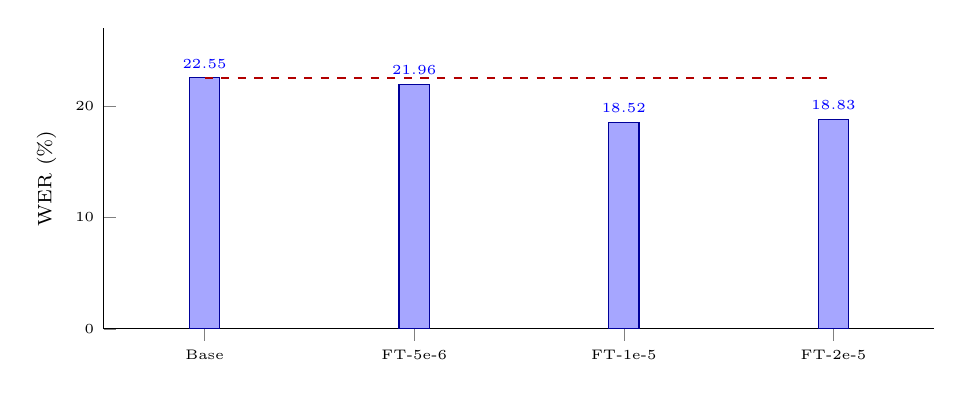
\begin{tikzpicture}
        \begin{axis}[
          ybar,
          bar width=11pt,
          width=\linewidth,
          height=5.4cm,
          ylabel={WER (\%)},
          ymin=0, ymax=27,
          symbolic x coords={Base, FT-5e-6, FT-1e-5, FT-2e-5},
          xtick=data,
          nodes near coords,
          nodes near coords style={font=\tiny},
          enlarge x limits=0.16,
          axis lines*=left,
          tick label style={font=\tiny},
          label style={font=\scriptsize},
        ]
          \addplot+[fill=blue!35, draw=blue!60!black] coordinates {
            (Base,22.55) (FT-5e-6,21.96) (FT-1e-5,18.52) (FT-2e-5,18.83)
          };
          \draw[red!70!black, dashed, thick]
            (axis cs:Base,22.55) -- (axis cs:FT-2e-5,22.55);
        \end{axis}
      \end{tikzpicture}
    \end{column}
  \end{columns}
\end{frame}

\begin{frame}{Results: Where the Improvement Comes From}
  \begin{columns}[T]
    \begin{column}{0.5\textwidth}
      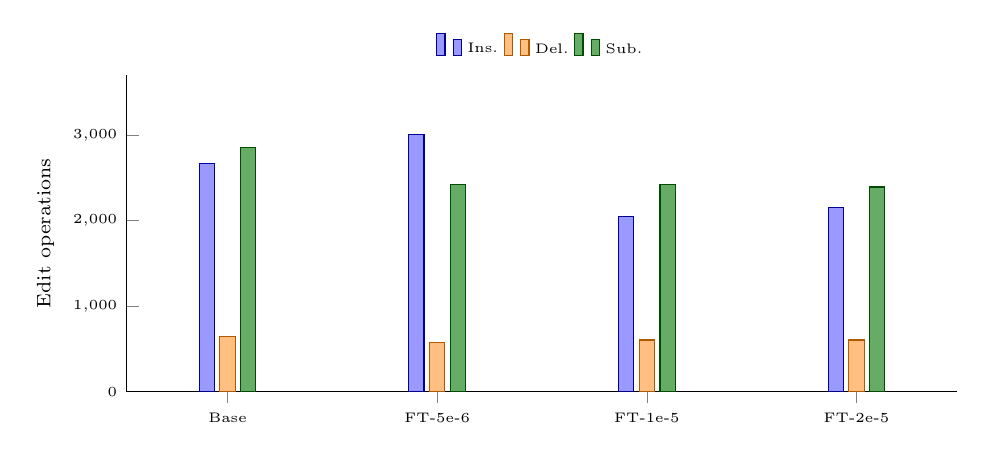
\begin{tikzpicture}
        \begin{axis}[
          ybar,
          bar width=5.5pt,
          width=\linewidth,
          height=5.6cm,
          ylabel={Edit operations},
          ymin=0, ymax=3700,
          symbolic x coords={Base, FT-5e-6, FT-1e-5, FT-2e-5},
          xtick=data,
          enlarge x limits=0.16,
          axis lines*=left,
          legend style={font=\tiny, at={(0.5,1.02)}, anchor=south, legend columns=3, draw=none},
          tick label style={font=\tiny},
          label style={font=\scriptsize},
        ]
          \addplot+[fill=blue!40, draw=blue!60!black] coordinates {
            (Base,2668) (FT-5e-6,3005) (FT-1e-5,2045) (FT-2e-5,2156)};
          \addplot+[fill=orange!50, draw=orange!70!black] coordinates {
            (Base,640) (FT-5e-6,577) (FT-1e-5,603) (FT-2e-5,604)};
          \addplot+[fill=green!45!black!60, draw=green!30!black] coordinates {
            (Base,2858) (FT-5e-6,2426) (FT-1e-5,2417) (FT-2e-5,2392)};
          \legend{Ins., Del., Sub.}
        \end{axis}
      \end{tikzpicture}
    \end{column}
    \begin{column}{0.46\textwidth}
      \begin{itemize}
        \item FT-1e-5 wins by producing \textbf{fewer extra words} (insertions: 2,668 $\rightarrow$ 2,045) and \textbf{fewer wrong words} (substitutions: 2,858 $\rightarrow$ 2,417).
        \item FT-2e-5 shows the same pattern, slightly behind on insertions.
        \item FT-5e-6 cut substitutions but its insertions rose to 3,005, absorbing most of the gain.
        \item A run can improve one error type while worsening another.
      \end{itemize}
    \end{column}
  \end{columns}
\end{frame}

\begin{frame}{Discussion}
  \begin{itemize}
    \item The learning rate controls a \textbf{tradeoff}: 1e-5 and 2e-5 buy intelligibility; 5e-6 stays closest to the base model's speaker similarity.
    \item FT-2e-5 shows the cost of pushing harder: nearly the same WER as FT-1e-5, but the \textbf{only SIM-o below base} (0.583).
    \item The base model keeps the highest UTMOS (3.64); fine-tunes are close at 3.60--3.61 --- a small, consistent naturalness cost.
    \item No single metric picks the winner; FT-1e-5 wins on the \textbf{overall pattern}: nearly all the WER gain with SIM-o preserved.
    \item Practical lessons: tokenize once and reuse; a conservative FP16 + gradient-accumulation recipe makes T4 training feasible.
  \end{itemize}
\end{frame}

\begin{frame}{Limitations}
  \begin{itemize}
    \item Automatic metrics only: WER is ASR-mediated (Whisper), SIM-o depends on the speaker encoder, UTMOS is a predictor, not a listening survey.
    \item Read speech only, with many short isolated-word prompts; says little about spontaneous speech or long-form prosody.
    \item Filipino only; other Philippine languages in PLD were not tested.
    \item Three learning-rate settings, not a full sweep, because of free-GPU compute limits.
  \end{itemize}
\end{frame}

\begin{frame}{Conclusion and Recommendations}
  \begin{block}{Answer to the Research Question}
    Filipino fine-tuning improved OmniVoice intelligibility: WER dropped from 22.55\% to 18.52\% (17.9\% relative) with speaker similarity preserved. The learning rate controls an intelligibility-versus-speaker-similarity tradeoff; no setting wins every metric.
  \end{block}

  \vspace{0.5em}

  \begin{itemize}
    \item Recommended checkpoint: \textbf{FT-1e-5} (best dev loss, found at step 4900).
    \item Next: Filipino listener study to validate the automatic metrics.
    \item Next: more learning rates around 1e-5; repeat runs across seeds.
    \item Next: curated sentence-level data to improve prosody.
  \end{itemize}
\end{frame}

\begin{frame}{Application Use Case: Voice Cloning}
  \centering
  
\includegraphics[width=0.94\linewidth,height=0.78\textheight,keepaspectratio]{\detokenize{../../../showcase-screenshot.png}}
\end{frame}

\begin{frame}{Public Showcase}
  \begin{columns}[T]
    \begin{column}{0.58\textwidth}
      \Large \textbf{OmniVoice Filipino Showcase}

      \vspace{0.8em}
      \normalsize
      Public demo for comparing reference audio, base OmniVoice, and Filipino fine-tuned outputs from the evaluation samples.

      \vspace{1.0em}
      \small
      \url{https://omnivoice-showcase.duncanb013.workers.dev/}
    \end{column}
    \begin{column}{0.34\textwidth}
      \centering
      
\includegraphics[width=0.82\linewidth,height=0.62\textheight,keepaspectratio]{\detokenize{../../../qrcode_omnivoice-showcase.duncanb013.workers.dev.png}}
    \end{column}
  \end{columns}
\end{frame}

\begin{frame}{References}
  \tiny
  \begin{itemize}
    \item Cajote, R. D., Guevara, R. C. L., Bayona, M. G. A. R., \& Lucas, C. R. G. (2024). \textit{Philippine Languages Database: A multilingual speech corpora for developing systems for Philippine spoken languages}. SIGUL 2024. \url{https://aclanthology.org/2024.sigul-1.32/}
    \item Le, M., Vyas, A., Shi, B., Karrer, B., Sari, L., Moritz, R., Williamson, M., Manohar, V., Adi, Y., Mahadeokar, J., et al. (2023). \textit{Voicebox: Text-guided multilingual universal speech generation at scale}. NeurIPS, 36, 14005--14034.
    \item Saeki, T., Xin, D., Nakata, W., Koriyama, T., Takamichi, S., \& Saruwatari, H. (2022). \textit{UTMOS: UTokyo-SaruLab system for VoiceMOS Challenge 2022}. Interspeech 2022. \url{https://arxiv.org/abs/2204.02152}
    \item UP EEEI - Digital Signal Processing Laboratory. (2026). \textit{UP-DSP Philippine Languages Database}. Mozilla Data Collective. \url{https://mozilladatacollective.com/datasets/cmmxhw46c00tqnw07xyr94zjk}
    \item Wang, C., Chen, S., Wu, Y., Zhang, Z., Zhou, L., Liu, S., et al. (2023). \textit{Neural codec language models are zero-shot text to speech synthesizers}. arXiv. \url{https://arxiv.org/abs/2301.02111}
    \item Zhu, H., Ye, L., Kang, W., Yao, Z., Guo, L., Kuang, F., Han, Z., Zhuang, W., Lin, L., \& Povey, D. (2026). \textit{OmniVoice: Towards omnilingual zero-shot text-to-speech with diffusion language models}. arXiv. \url{https://arxiv.org/abs/2604.00688}
    \item Weights \& Biases experiment report: \url{https://wandb.ai/duncanb013-polytechnic-university-of-the-philippines/OmniVoice-PLD-Filipino}
  \end{itemize}
\end{frame}

\end{document}
